\begin{table*}[t]
\centering
% \vspace{-1ex}
\renewcommand\arraystretch{0.93}
\caption{Main results (acc\%) on five in-distribution and six out-of-distribution VQA benchmarks. $^\dagger$ indicates results reported from the original papers. 
\emph{w/o Tools} excludes tool access from both training and inference stage; \emph{w/o Reasoning} removes RL training stage.
}
% \vspace{-1ex}
\resizebox{1.0\linewidth}{!}{ %
\begin{tabular}{l @{\hskip2.5pt} | c c c c c | c | c c c c c c  | c | c c }
\toprule
\textbf{Baselines ($\downarrow$)} &  \multicolumn{6}{c|}{\textbf{In-Distribution}} & \multicolumn{7}{c|}{\textbf{Out-of-Distribution}} & \textbf{All} \\
\cmidrule(lr){2-7} \cmidrule(lr){8-14} \cmidrule(lr){15-15}
\textbf{Datasets ($\rightarrow)$} & ChartQA & Geometry3K & GeoQA & UniGeo & MapQA & avg. & TABMWP & AI2D & PlotQA & CLEVR-Math & IconQA & MathVista  &  avg. &  avg.  \\
\midrule
\multicolumn{10}{l}{\textit{Commercial VLMs (For reference)}} \\
\midrule
%%%%%%%%%%%%%%%%%%%%%%%%%%%%%%%%%%%%%%
GPT-5 & 85.92 &	94.84 &	90.91 &	49.34 &	60.95 &	76.39 &	99.90 &	86.10 &	72.90 &	26.00 &	87.20 &	80.20 &	75.38 &	75.84 \\
GPT-5-mini & 82.80 &	91.01 &	88.01 &	46.02 &	61.35 &	73.84 &	98.57 &	85.85 &	70.95 &	27.15 &	87.73 & 79.30 &	74.93 &	74.43\\
GPT-o4-mini & 85.24 &	90.02 &	89.17 &	40.72 &	62.25 &	73.48 &	96.73 &	84.38 &	73.35 &	27.35 &	86.53 &	78.00 &	74.39 &	73.98 \\ 
GPT-o3 & 85.63 &	92.35 &	90.14 &	50.27 &	54.25 &	74.53 &	99.18 &	79.58 &	71.85 &	25.55 &	81.87 &	75.40 &	72.24 &	73.28 \\ 
Gemini-2.5-Pro & 83.64 & 94.34 & 86.85 & 60.34 & 64.20 &	77.87 &	99.90 &	90.28 &	77.40 &	25.70 &	96.93 & 82.00 &	78.70 &	78.33 \\
Gemini-2.5-Flash & 85.85 &	92.85 &	88.78 &	46.15 &	53.35 &	73.40 &	97.96 &	84.50 &	68.75 &	23.45 &	84.73 &	77.90 &	72.88 &	73.12 \\
Claude-4.5-Sonnet & 85.03 &	85.19 &	92.26 &	55.57 &	91.85 &	81.98 &	99.49 &	80.44 &	82.95 &	23.95 &	94.50 &	75.10 &	76.07	& 78.76 \\
\midrule
%%%%%%%%%%%%%%%%%%%%%%%%%%%%%%%%%%%%%%
\multicolumn{10}{l}{\textit{Base Size: < 7B parameters}} \\
\midrule
InternVL3-2B   & 24.08  &	40.26  &	40.21  &	21.88  &	16.35  &	28.56  &	82.41  &	63.59  &	38.94  &	17.90  &	60.13  &	32.70  &	49.28  &	39.86 \\
\rowcolor{magenta!12} \ours{} (InternVL3-2B) &  88.55 &	56.24 &	68.54 &	42.31 &	33.35 &	57.80 &	85.35 &	73.80 &	63.85 &	39.81 &	84.13 &	60.00 &	67.82 &	63.27 \\
\rowcolor{magenta!3} \quad w/o Tools  &	72.88  &	43.93  &	66.30  &	39.52  &	39.45  &	52.42  &	74.23  &	64.70  &	35.90  &	15.93  &	63.53  &	49.60  &	50.65  &	51.45 \\
\rowcolor{magenta!3} \quad w/o Reasoning & 43.76	& 43.43	& 54.93	& 23.47 &	25.05 &	38.13 &	85.27 &	51.29 &	30.85 &	21.24 &	68.53 &	28.30 & 47.58 &	43.28 	\\
Qwen2.5-VL-3B  & 40.08  &	38.09  &	34.40  &	19.00  &	18.00  &	29.91  &	82.05  &	64.69  &	40.02  &	23.07  &	41.00  &	34.60  &	47.57  &	39.51 \\
LLaVA‑OneVision-1.5-4B 	& 61.60	&	50.92	&	29.79	&	14.06	&	27.25	&	36.72	&	93.15	&	73.68	&	43.90	&	24.00	&	84.80	&	44.50	&	60.67	&	49.79\\
\midrule
%%%%%%%%%%%%%%%%%%%%%%%%%%%%%%%%%%%%%%
\multicolumn{10}{l}{\textit{Large Size: 7 - 13B parameters}}  \\
\midrule
Qwen2.5-VL-7B & 76.40 &	39.43 &	41.39 &	30.64 &	26.30 &	42.83 &	80.64 &	70.44 &	65.53 &	25.18 &	61.45 &	59.20 &	60.41 &	52.42 \\
\rowcolor{teal!15}  \ours{} (Qwen2.5-VL-7B) & 90.08 &	53.27 & 71.32 &	44.43 &	66.85 &	65.19 &	86.40 &	72.68 &	74.82 &	33.37 &	72.51 &	63.00 &	67.13 &	66.25  \\ 
\rowcolor{teal!4}  \quad w/o Tools & 83.32 &	48.92 &	68.11 &	33.42 &	51.35 &	57.02 &	64.13 &	56.09 &	76.45 &	26.92 &	68.58 &	56.10 &	58.05 &	57.58 \\	
\rowcolor{teal!4}  \quad w/o Reasoning & 79.68 &	47.92 &	58.61 &	34.88 &	26.70 &	49.56 &	82.11 &	72.09 &	66.90 &	17.93 &	82.87 &	42.50 &	60.73 &	55.65 \\					
VTool-R1-7B & 80.70$^\dagger$ & 62.06 &	65.18 &	33.29 &	19.65 &	52.18 &	64.21 &	79.34 &	48.85 &	19.70 &	75.67 &	36.60 &	54.06 &	53.20 \\
R1‑VL‑7B & 83.90$^\dagger$ &	58.90 &	62.09 &	37.93 &	23.87 &	57.34 &	92.64 &	76.51 &	48.50 &	18.00 &	87.27 &	63.50$^\dagger$ & 65.20 & 61.63 \\
R1‑Onevision‑7B  &59.92 &	55.79 &	57.47 &	28.30 &	33.20 &	46.94 &	84.19 &	61.75 &	35.40 &	19.30 &	79.30 &	64.10 &	57.34 &	52.61 \\	
Perception‑R1-7B & 	76.41 &	48.59 &	51.23 &	21.22 &	40.52 &	47.59 &	84.05 &	67.77 &	44.30 &	18.00 &	81.87 & 74.20$^\dagger$ &	61.70	& 55.29 \\	
InternVL3-8B   & 77.32 & 47.09 &	44.87 &	33.71 &	34.70 &	47.54 &	95.32 &	74.54 &	63.05 &	28.95 &	73.27 &	59.60 &	65.79 &	57.49 \\ 
\rowcolor{teal!15}  \ours{} (InternVL3-8B) &  91.92 &	61.27 &	76.41 &	49.67 &	68.45 &	69.54 &	96.52 &	79.86 &	66.38 &	38.20 &	91.09 &	62.80 &	72.48 &	71.14 \\ 
\rowcolor{teal!4}  \quad w/o Tool  & 84.24 &	51.47 &	73.10 &	34.70 &	53.50 &	59.40 &	94.68 &	75.37 &	60.25 &	29.24 &	80.93 &	62.80 &	67.21 &	63.66 \\
\rowcolor{teal!4}  \quad w/o Reasoning  & 68.56 & 35.64 &	55.90 &	27.06 &	26.45 &	42.72 &	92.34 &	50.45 &	38.70 &	28.18 &	80.07 &	29.10 &	53.14 &	48.40 \\ 
LLaVA‑OneVision-1.5-8B & 64.96 & 54.08 & 32.69 & 16.05 & 32.40 & 40.04 &	94.27 &	77.37 &	46.60 &	25.00 &	89.67 &	47.70 &	63.44 &	52.80 \\
\midrule
%%%%%%%%%%%%%%%%%%%%%%%%%%%%%%%%%%%%%%
\multicolumn{10}{l}{\textit{XL Size: > 13B parameters}}  \\
\midrule
InternVL3-14B &  87.30 &	68.89 &	75.05 &	41.78 &	50.77 &	64.76 &	97.71 &	75.40 &	74.12 &	32.83 &	81.47 &	71.67 &	72.20 &	68.82 \\
\rowcolor{blue!12}  \ours{} (InternVL3-14B) & 93.60 &	83.87 &	78.85 &	52.94 &	70.50 &	75.95 &	98.02 &	87.60 &	76.00 &	40.86 &	92.13 &	68.00 &	77.10 &	76.58   \\
Qwen2.5-VL-32B  & 87.30&	65.22&	50.29&	42.94&	89.20&	66.99&	94.79&	82.16&	71.17&	35.14&	92.60&	68.20&	74.01&	70.82	 \\
InternVL3-38B &  89.20 &	70.72 &	79.11 &	45.14 &	55.13 &	67.86 &	98.35 &	83.03 &	78.48 &	33.88 &	83.73 &	74.03 &	75.25 &	71.89 \\
InternVL3-78B  & 89.70&	78.76&	85.43&	53.40&	58.15&	73.09&	99.39&	85.85&	82.35&	25.15&	86.33&	78.80&	76.31& 74.85 \\
% \midrule
%%%%%%%%%%%%%%%%%%%%%%%%%%%%%%%%%%%%%%
% \multicolumn{10}{l}{\textit{Tool-Integrated Reasoning Baselines (For reference)}}  \\
% \midrule

% \midrule
% %%%%%%%%%%%%%%%%%%%%%%%%%%%%%%%%%%%%%%
% \multicolumn{10}{l}{\textit{Reasoning-Only Baselines (For reference)}}  \\
% \midrule

\bottomrule
\end{tabular}%
}
\label{tab:main_results}
\end{table*}

\section{Experiments}
\label{sec:exp}

\subsection{Experiment Setups}
\noindent \textbf{Evaluation Datasets.}
Following several prior works \cite{liu2025visionreasoner,huang2025vision,han2025tiger,li2025self}, we focus on \emph{reasoning-intensive VQA tasks}, evaluating the effectiveness of \env{} in improving the TIR of open-source VLMs.
For \emph{in‑distribution} evaluation, we select five out of the thirteen datasets in \env{} training pool with official held-out test splits: (1) ChartQA~\cite{masry2022chartqa}, (2) Geometry3K~\cite{lu2021inter}, (3) GeoQA~\cite{chen2021geoqa}, (4) UniGeo~\cite{chen2022unigeo}, and (5) MapQA~\cite{chang2022mapqa}. 
To assess \emph{out‑of‑distribution} generalization, we evaluate on six additional benchmarks not used for training: (6) TABMWP~\cite{lu2022dynamic}, (7) AI2D~\cite{kembhavi2016diagram}, (8) PlotQA~\cite{methani2020plotqa}, (9) CLEVR-Math~\cite{lindstrom2022clevr}, (10) IconQA~\cite{lu2021iconqa}, and (11) MathVista~\cite{lu2023mathvista}.
Detailed dataset information is in Appendix \ref{app:data}.

\noindent \textbf{Baselines.}
We consider the following baselines on \env{}:
(i) \emph{API-based proprietary VLMs}, including GPT-5~\cite{gpt5}, GPT-5-mini~\cite{gpt5}, GPT-o4-mini~\cite{openai2025introducing}, GPT-o3~\cite{openai2025introducing}, Gemini-2.5-Pro~\cite{comanici2025gemini}, Gemini-2.5-Flash~\cite{comanici2025gemini}, Claude-4.5-Sonnet~\cite{Claude};
(ii) \emph{Open-source VLMs}, including InternVL3~\cite{zhu2025internvl3}, Qwen2.5-VL~\cite{bai2025qwen2}, LLaVA-OneVision-1.5~\cite{an2025llava};
(iii) \emph{Tool/Reasoning-integrated VLMs}, including VTool-R1~\cite{wu2025vtool}, R1-VL~\cite{zhang2025r1}, R1-Onevision~\cite{yang2025r1}, Perception-R1~\cite{yu2025perception}.
All baselines are evaluated \emph{without tool access}, as naive tool exposure significantly degrades performance without extensive agentic training (see Table~\ref{tab:fig-tir}); except for tool-integrated baselines following their original tool configurations.
Additional baseline details are available in Appendix~\ref{app:baseline}.

\noindent \textbf{Implementation Details.}
We consider four different backbones for \ours{} with varying sizes, including InternVL3-2B/8B/14B and Qwen2.5-VL-7B, and implement training with Verl-Tool~\cite{jiang2025verltool}. 
For SFT, we train for one epoch with a batch size of 128, a learning rate of $2\times10^{-6}$, and a context length of 16,384 tokens.
For RL, we use a micro-batch size of 8 per GPU, a mini-batch size of 128, and $G=8$ rollouts per update. We set the regularization coefficient $\beta=10^{-3}$, cap the maximum response length at 26,780 tokens, and optimize with a learning rate of $5\times10^{-7}$ for $E=300$ steps.
We adopt \emph{accuracy} (ACC) as the primary evaluation metric. All experiments are conducted with 8 NVIDIA H200 GPUs, each equipped with 141GB of memory.
See Appendix~\ref{app:prompt} and \ref{app:implementation} for prompt templates and other implementation details, respectively.



\subsection{Main Experiment Results}
Table~\ref{tab:main_results} shows the main results of \ours{} trained in \env{} against baselines on eleven visual‑reasoning datasets. From the results, we have the following key observations:
\textbf{(i) \ours{} achieves strong performance over baselines.} Notably, \ours{}-8B outperforms baselines with similar sizes by 9.51\%-18.72\% with tools and 2.03\%-11.24\% even \emph{without} tools, respectively.
\textbf{(ii) RL is critical for boosting TIR in VLMs.} Simply augmenting VLMs with tools without explicit reasoning supervision degrades accuracy. By contrast, RL delivers substantial gains, indicating that base checkpoints do not exhibit robust TIR ability and that RL is crucial for unlocking tool‑use capabilities in visual reasoning. Moreover, RL confers strong generalization: 
for example, \ours{}-8B attains accuracy on out‑of‑distribution VQA benchmarks comparable to substantially larger proprietary models (\eg, GPT‑o3 and Claude‑4.5‑Sonnet).
\textbf{(iii) \ours{} has a strong parameter efficiency.}
\ours{}-2B achieves competitive or even better performance with 8B baselines, while \ours{}-8B performs comparably to baselines with 38B parameters. 
The superiority of \ours{} demonstrates that \textbf{\env{} provides a scalable training ground for tool‑integrated agentic RL}, enabling robust visual reasoning in open‑source VLMs.

\begin{figure*}[t]
    \centering
    % \vspace{-2ex}
    \begin{subfigure}[t]{0.33\linewidth}
        \centering
        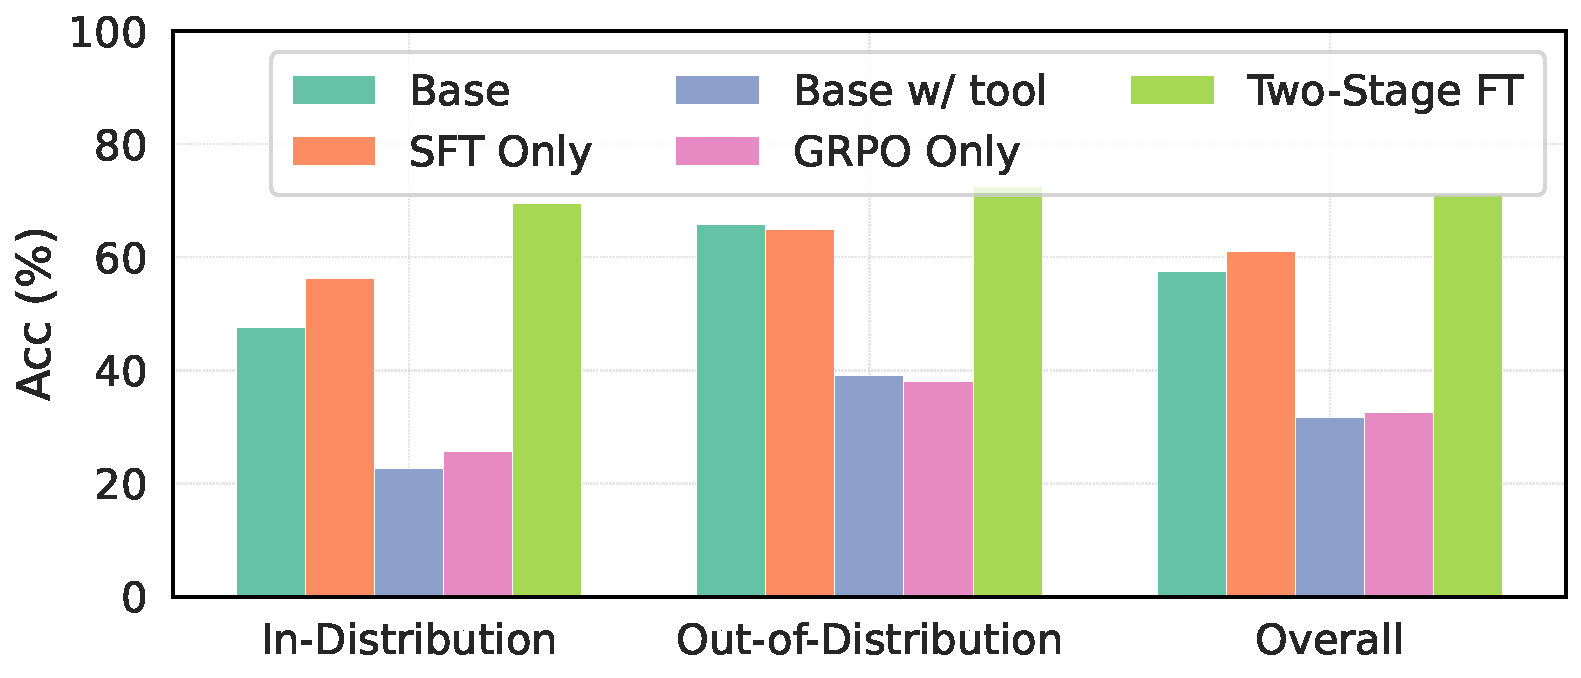
\includegraphics[width=\linewidth]{figure/effect-of-training-stage.pdf}
        \caption{Effect of training stages}
        \label{fig:abl-training}
    \end{subfigure}
    \hfill
    \begin{subfigure}[t]{0.33\linewidth}
        \centering
        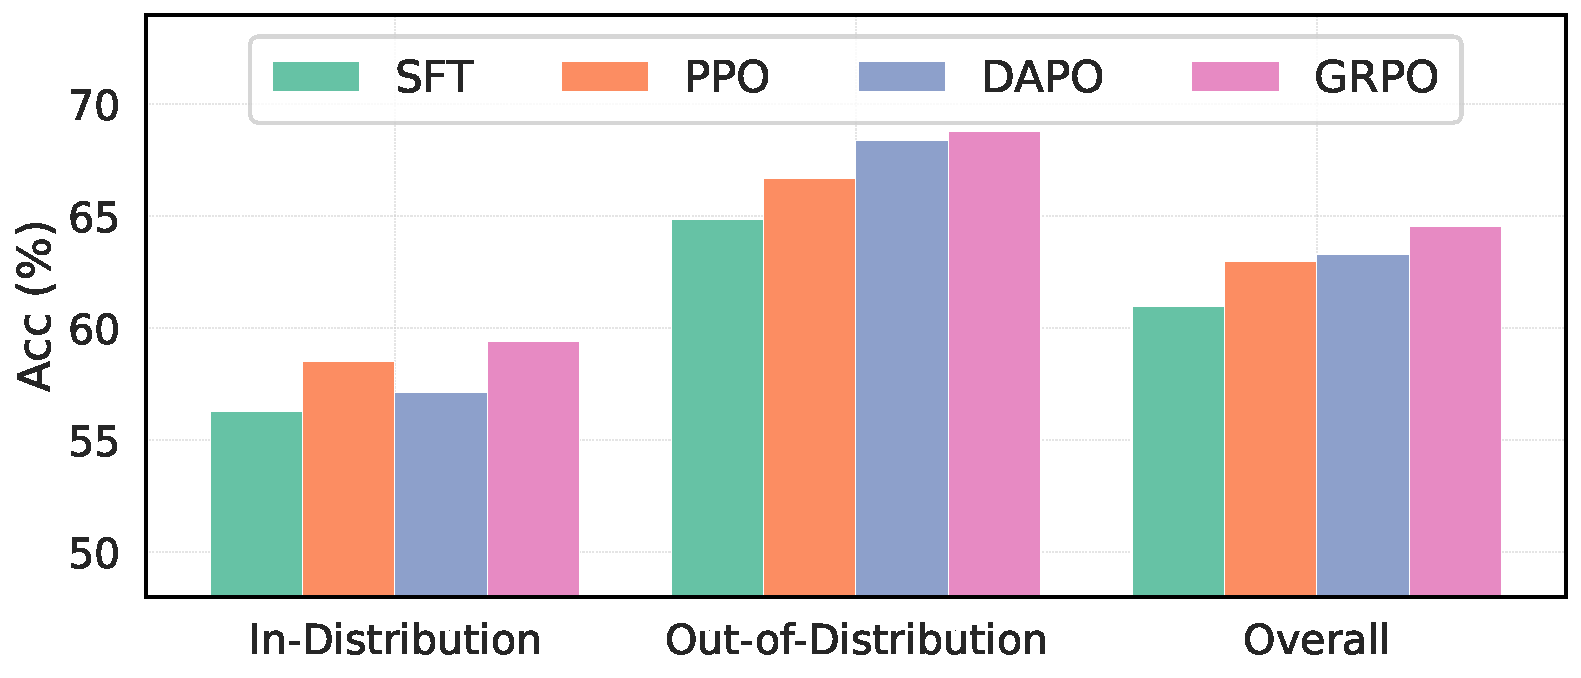
\includegraphics[width=\linewidth]{figure/effect-of-RL-method.pdf}
        \caption{Effect of RL algorithms ($E$=100)}
        \label{fig:abl-rl}
    \end{subfigure}
    \hfill
    \begin{subfigure}[t]{0.33\linewidth}
        \centering
        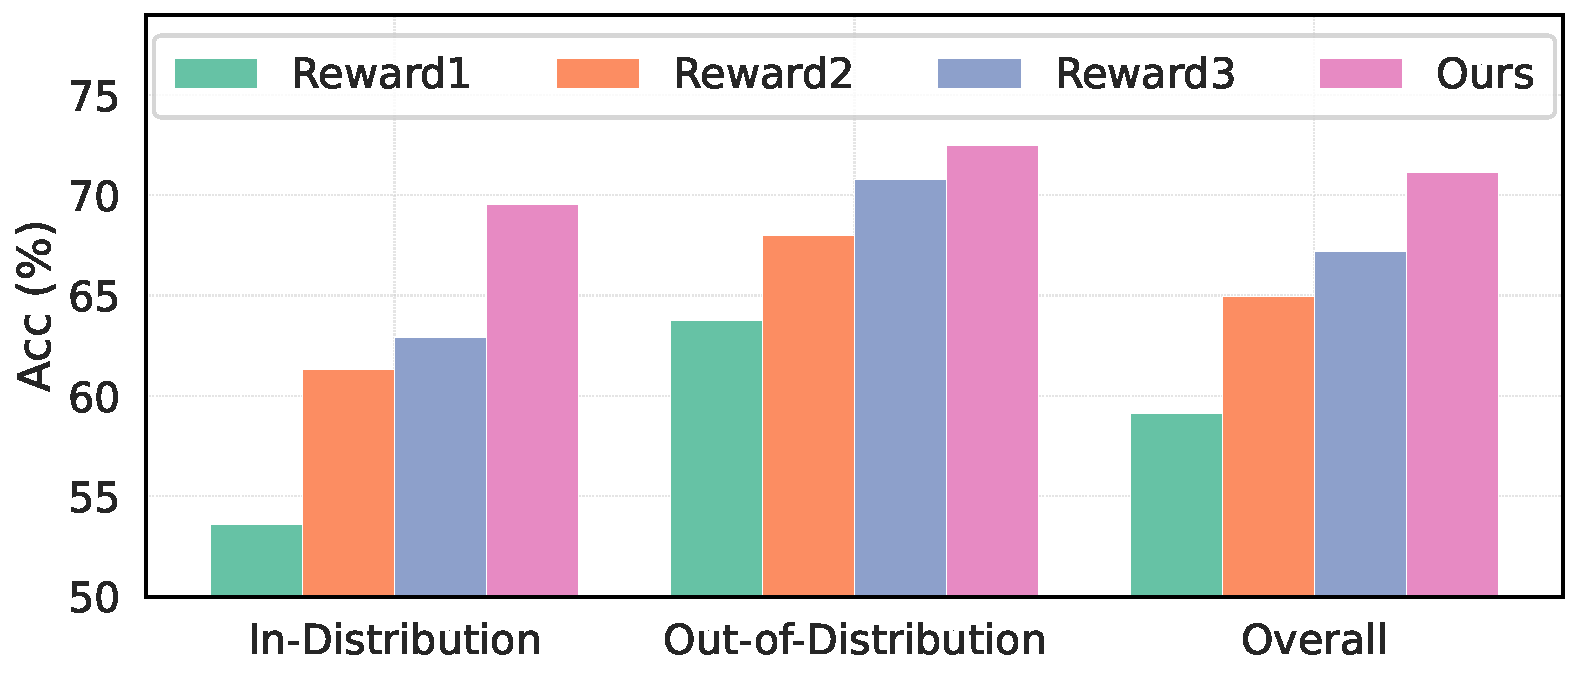
\includegraphics[width=\linewidth]{figure/effect-of-Reward.pdf}
        \caption{Effect of reward design}
        \label{fig:abl-reward}
    \end{subfigure}
       \hfill
        \begin{subfigure}[t]{0.33\linewidth}
        \centering
        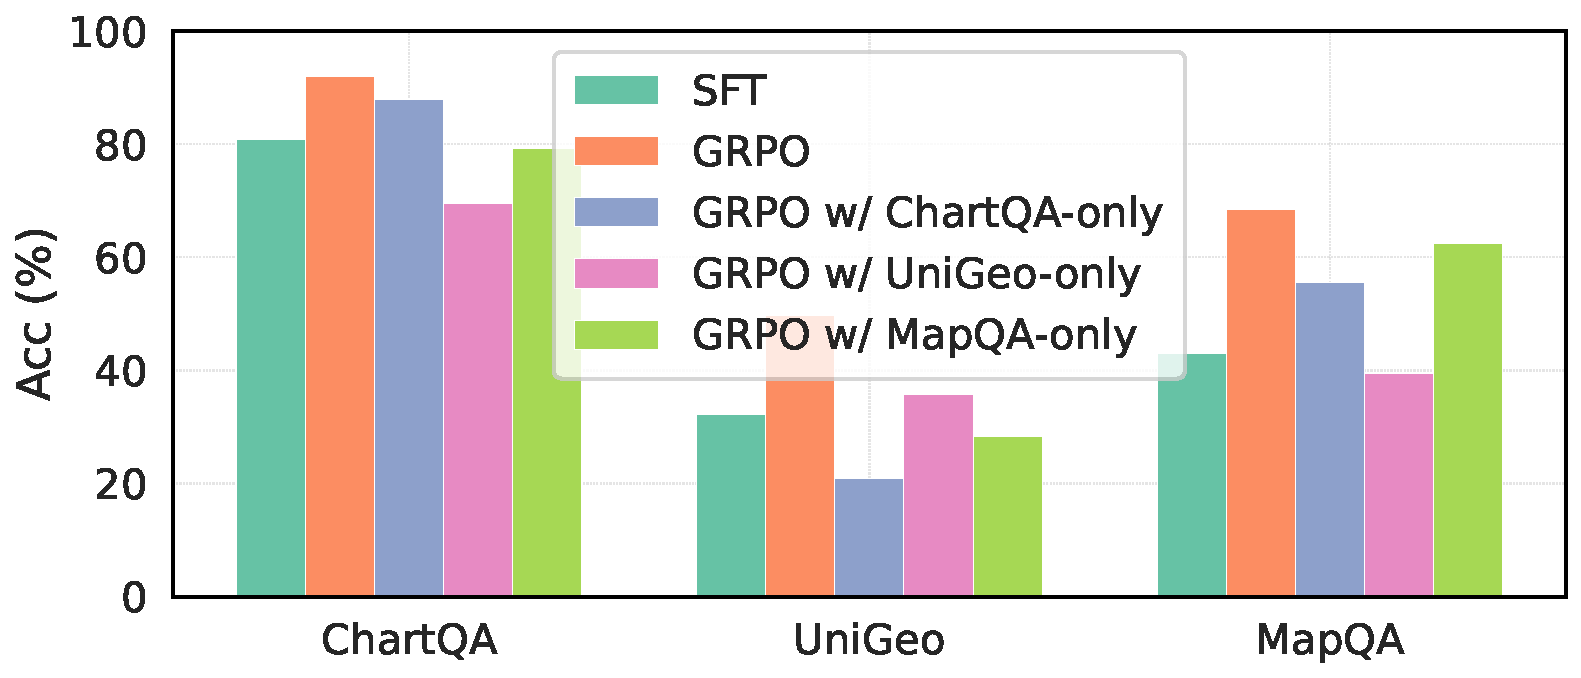
\includegraphics[width=\linewidth]{figure/effect-of-data-diversity.pdf}
        \caption{Effect of data diversity}
        \label{fig:adata-diversity}
    \end{subfigure}
    \hfill
    \begin{subfigure}[t]{0.33\linewidth}
        \centering
        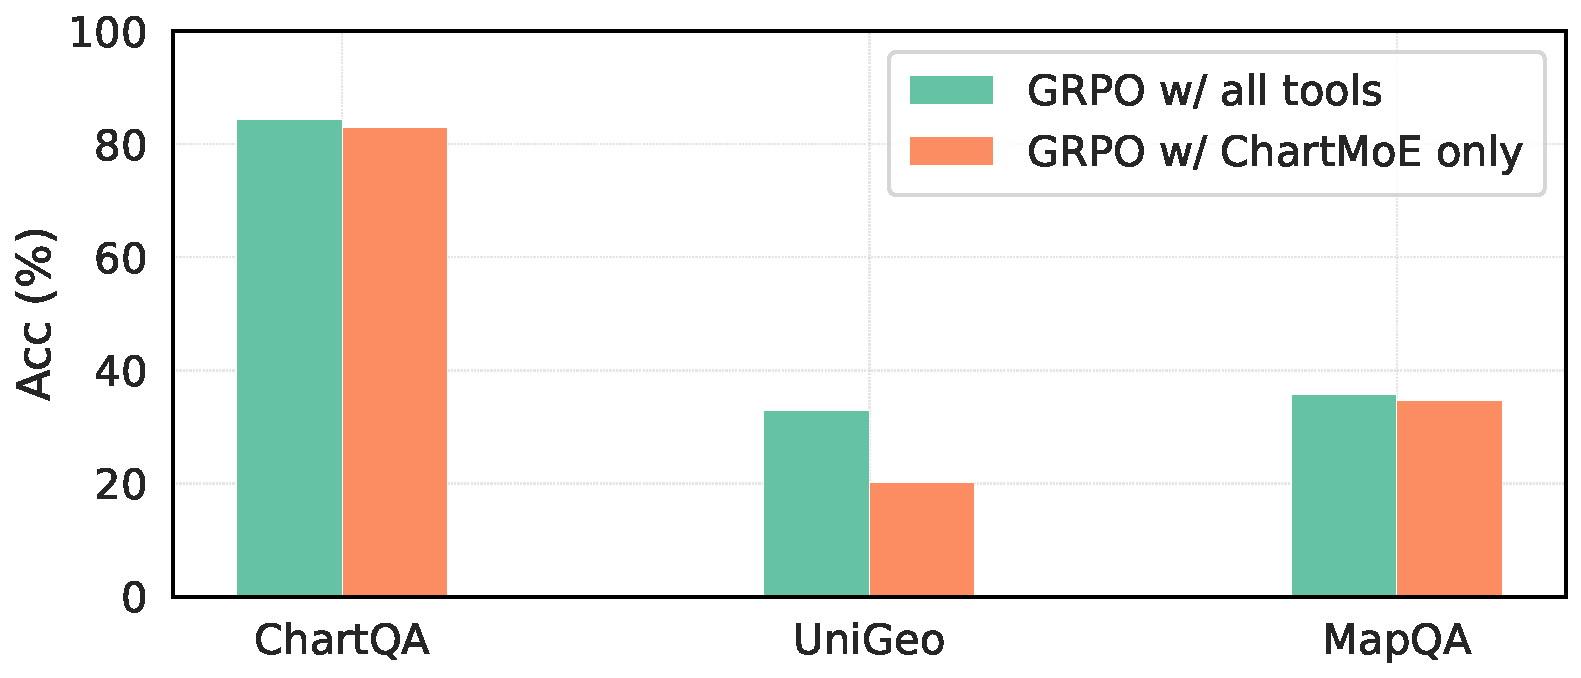
\includegraphics[width=\linewidth]{figure/effect-of-tool-diversity.pdf}
        \caption{Effect of tool diversity ($E$=50)}
        \label{fig:tool-diversity}
    \end{subfigure}
    \hfill
    \begin{subfigure}[t]{0.33\linewidth}
        \centering
        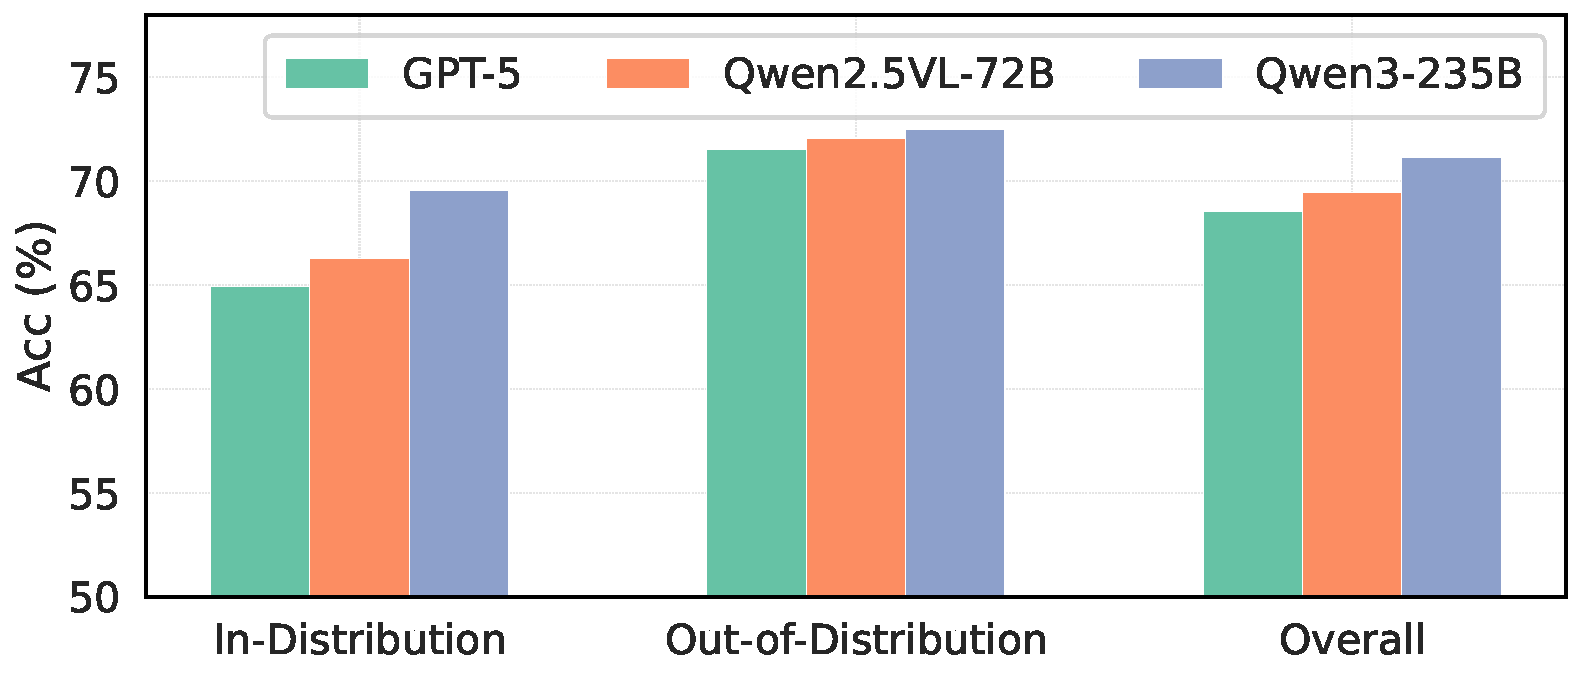
\includegraphics[width=\linewidth]{figure/effect-of-traj-quality.pdf}
        \caption{Effect of thinking trajectory quality}
        \label{fig:effect-of-traj-quality}
    \end{subfigure}
    \caption{Ablation studies and diversity analysis with InternVL3-8B as backbone VLM.}
    % \vspace{-1ex}
    \label{fig:ablation-study}
\end{figure*}

\begin{table*}[t]
\centering
\renewcommand\arraystretch{0.93}
% \vspace{-2ex}
\caption{Effect of reasoning and tool-use results without RL training. \emph{w/ Tools} refers to directly augmenting VLMs with tools significantly degrades accuracy; \emph{w/ Reasoning} refers to CoT reasoning without tools. \emph{w/ T\&R} refers to a different setting compared to TIR, only supplying \emph{tool‑selection prior knowledge} and interleaving reasoning with tool execution improve performance. }
\resizebox{1.0\linewidth}{!}{ %
\begin{tabular}{l @{\hskip2.5pt} | c c c c c | c | c c c c c c  | c | c c }
\toprule
\textbf{Baselines ($\downarrow$)} &  \multicolumn{6}{c|}{\textbf{In-Distribution}} & \multicolumn{7}{c|}{\textbf{Out-of-Distribution}} & \textbf{All} \\
\cmidrule(lr){2-7} \cmidrule(lr){8-14} \cmidrule(lr){15-15}
\textbf{Datasets ($\rightarrow)$} & ChartQA & Geometry3K & GeoQA & UniGeo & MapQA & avg. & TABMWP & AI2D & PlotQA & CLEVR-Math & IconQA & MathVista  &  avg. &  avg.  \\
\midrule
\rowcolor{gray!15}  GPT-5 & 85.92 &	94.84 &	90.91 &	49.34 &	60.95 &	76.39 &	99.90 &	86.10 &	72.90 &	26.00 &	87.20 &	80.20 &	75.38 &	75.84 \\
\quad w/ Tools & 58.60 & 74.04 & 65.00 & 28.78& 31.20 & 51.52 &69.83 & 65.07 & 46.75 & 18.96 & 60.53 & 42.60 & 50.62 & 51.03\\
\quad w/ Reasoning  & 85.68 & 91.01 & 86.27 & 51.25& 59.48 & 74.74 &99.81 & 83.03 & 84.73& 25.50 & 86.27 & 80.90 & 76.71 & 75.81\\
\quad w/ T\&R &  94.00 & 93.84 & 91.56 & 51.69 & 57.35& 77.69 & 98.92 & 84.62& 79.45 & 27.79& 91.07 & 57.80 & 73.28 & 75.28 \\
\midrule
\rowcolor{gray!15}  InternVL3-8B   & 77.32 & 47.09 &	44.87 &	33.71 &	34.70 &	47.54 &	95.32 &	74.54 &	63.05 &	28.95 &	73.27 &	59.60 &	65.79 &	57.49 \\ 
\quad w/ Tools & 25.44 &  17.06& 27.27 & 26.90& 16.22 & 22.58 &58.15 & 51.74 & 58.31 & 18.01 & 25.86 &  22.70& 39.13 & 31.61\\
\quad w/ Reasoning  & 81.28& 47.09 & 45.07 & 35.81&31.10 &  48.07& 94.38&76.51 & 65.85& 24.15 &75.53  &60.70  & 66.19 &57.95\\
\quad w/ T\&R & 68.56 & 35.64 & 55.90& 27.06 & 26.45&42.72 & 92.34 & 50.45& 38.70& 28.18& 80.07& 29.10& 53.14 &48.40 \\
% \midrule
% \rowcolor{gray!15}  InternVL3-2B   & 24.08  &	40.26  &	40.21  &	21.88  &	16.35  &	28.56  &	82.41  &	63.59  &	38.94  &	17.90  &	60.13  &	32.70  &	49.28  &	39.86 \\
% \quad w/ Tools & 19.20& 7.65 & 23.02 & 19.23& 8.45 & 15.51 & 34.00& 17.72& 29.05 & 1.81 & 25.40 & 21.70 & 21.61 & 18.84\\
% \quad w/ Reasoning  & 69.28 & 43.59 &42.82  &24.14 & 20.10& 39.99 & 87.88& 63.71 &43.25 &19.35 & 68.19 & 52.00 &55.73  & 48.57\\
% \quad w/ T\&R & 43.76  &43.43 &54.93  & 23.47 & 25.05& 38.13 & 85.27 &51.29 & 30.85 & 21.24& 68.53 & 28.30 & 47.59 & 43.28 \\
\bottomrule
\end{tabular}%
% \vspace{-2ex}
}
\label{tab:fig-tir}
\end{table*}


\subsection{Ablation Studies of \ours{}}
\noindent \textbf{Effect of Tool-Integrated Reasoning.}
Table~\ref{tab:main_results} also disentangles the roles of \emph{reasoning} and \emph{tool use} by reporting three variants: 
(1) \emph{w/o Tools} (63.66\%) that enables reasoning but disables tool access; 
(2) \emph{w/o Reasoning} (48.40\%) that exposes tools (with prior tool selection knowledge) without reinforcing reasoning; 
(3) and the \emph{full} \ours{} (71.14\%) that interleaves both. 
While strengthening reasoning or tool-use alone sometimes yields measurable gains, it remains suboptimal compared to \ours{}, which synergistically couples reasoning with tool execution.
Two key findings follow:
(i) simply exposing tools can be \emph{detrimental without sufficient reasoning} to navigate the action space, and
(ii) optimal problem solving arises when reasoning \emph{guides} (\emph{if/when/which}) tool invocation in an interleaved loop, rather than relying on either capability in isolation.

\noindent \textbf{Effect of Training Stage.}
Figure~\ref{fig:abl-training} shows that SFT serves as a critical \emph{warm-up}, aligning the model with tool-use formats and syntax (+3.46\%); RL then unlocks substantially larger gains (+10.19\% over SFT).
\emph{Both stages contribute}: SFT establishes the necessary behavioral priors for reliable tool interaction, while RL triggers deeper, interleaved reasoning required to navigate complex tasks effectively.

\noindent \textbf{Effect of RL Algorithm.}
In addition to GRPO, we evaluate PPO~\cite{schulman2017proximal} and DAPO~\cite{yu2025dapo} as preference-optimization algorithms; yet we observe that GRPO delivers the most robust performance, as shown in Figure~\ref{fig:abl-rl}.
The DAPO deficit may be due to the elimination of \emph{uniform‐reward} groups in its preference objective: in early stage, removing all-incorrect collapses the effective batch and starves the policy of learning signal; in later stage, removing all-correct erases useful supervision for reasoning–tool coordination. 
In contrast, GRPO retains all rollouts and uses group‑normalized advantages to deliver low‑variance, difficulty‑adaptive credit assignment, yielding more robust gains
% We attribute DAPO's performance deficit to its exclusion of sample groups with uniform outcomes. Specifically, by discarding "all-correct" groups, DAPO ignores successful but potentially suboptimal trajectories (e.g., those exhibiting tool over-reliance), thereby forfeiting the opportunity to refine the reasoning-tool synergy. Furthermore, in the early stages of RL where "all-incorrect" rollouts are prevalent due to the model's nascent capabilities, DAPO's filtering criteria result in severe data scarcity. In contrast, GRPO leverages relative advantages even within these uniform groups, maintaining a dense supervision signal essential for robust optimization.
% We hypothesize that DAPO's performance deficit stems from its exclusion of "all-correct" sample groups; while these trajectories achieve the correct outcome, they often exhibit tool over-reliance at the expense of reasoning depth, and discarding them removes critical supervision needed to further optimize the reasoning-tool synergy.
% Besides, at early stage of RL, the model capabilities in tool-use and reasoning are still weak, leading to rollouts all fail. 
% Removing them directly will only leave small proportion data to learn for the agent.

\noindent \textbf{Effect of Reward Design.}
Figure~\ref{fig:abl-reward} compares different types of reward design, including (1) dense reward $R_{\text{dense}}=-1+0.5R_{\text{format}}+0.5R_{\text{correct}}+R_{\text{format}}\cdot R_{\text{correct}}$, (2) sparse reward $R_{\text{sparse}}=R_{\text{format}}\cdot R_{\text{correct}}$, (3) difficulty-adaptive reward $R_{\text{diff}}=R\cdot w$, where $w=\text{clamp}(2-D,0,1)\times0.5+0.5$ and $D$ represents the difficulty measured by the mean base reward across all rollouts, $D=\mathbb{E}[R]$, and (4) ours.
In comparison, our reward design couples a \emph{verifiable, low‑noise binary end signal with difficulty‑adaptive scaling} via group‑normalized advantages, yielding superior accuracy while avoiding overfitting to easy cases or exploitation of intermediate signals. 

\noindent \textbf{Effect of Tool and Reasoning in Vanilla VLMs.}
Table~\ref{tab:fig-tir} summarizes the effect of tools and reasoning on vanilla VLMs for open- and closed-source models. Directly augmenting VLMs with tools significantly degrades accuracy, and intrinsic chain-of-thought alone yields only modest gains on complex VQA. Supplying \emph{tool-selection priors} improves performance; however, gains are strongly task-dependent for commercial VLMs, and smaller open-source VLMs remain particularly challenged. These observations underscore that it is both important and non-trivial to endow VLMs with robust, generalizable tool-use capabilities that adapt across diverse visual reasoning scenarios. 

\begin{figure*}[t]
    \centering
    % \vspace{-1ex}
    \begin{minipage}[t]{0.72\linewidth}
        \centering
        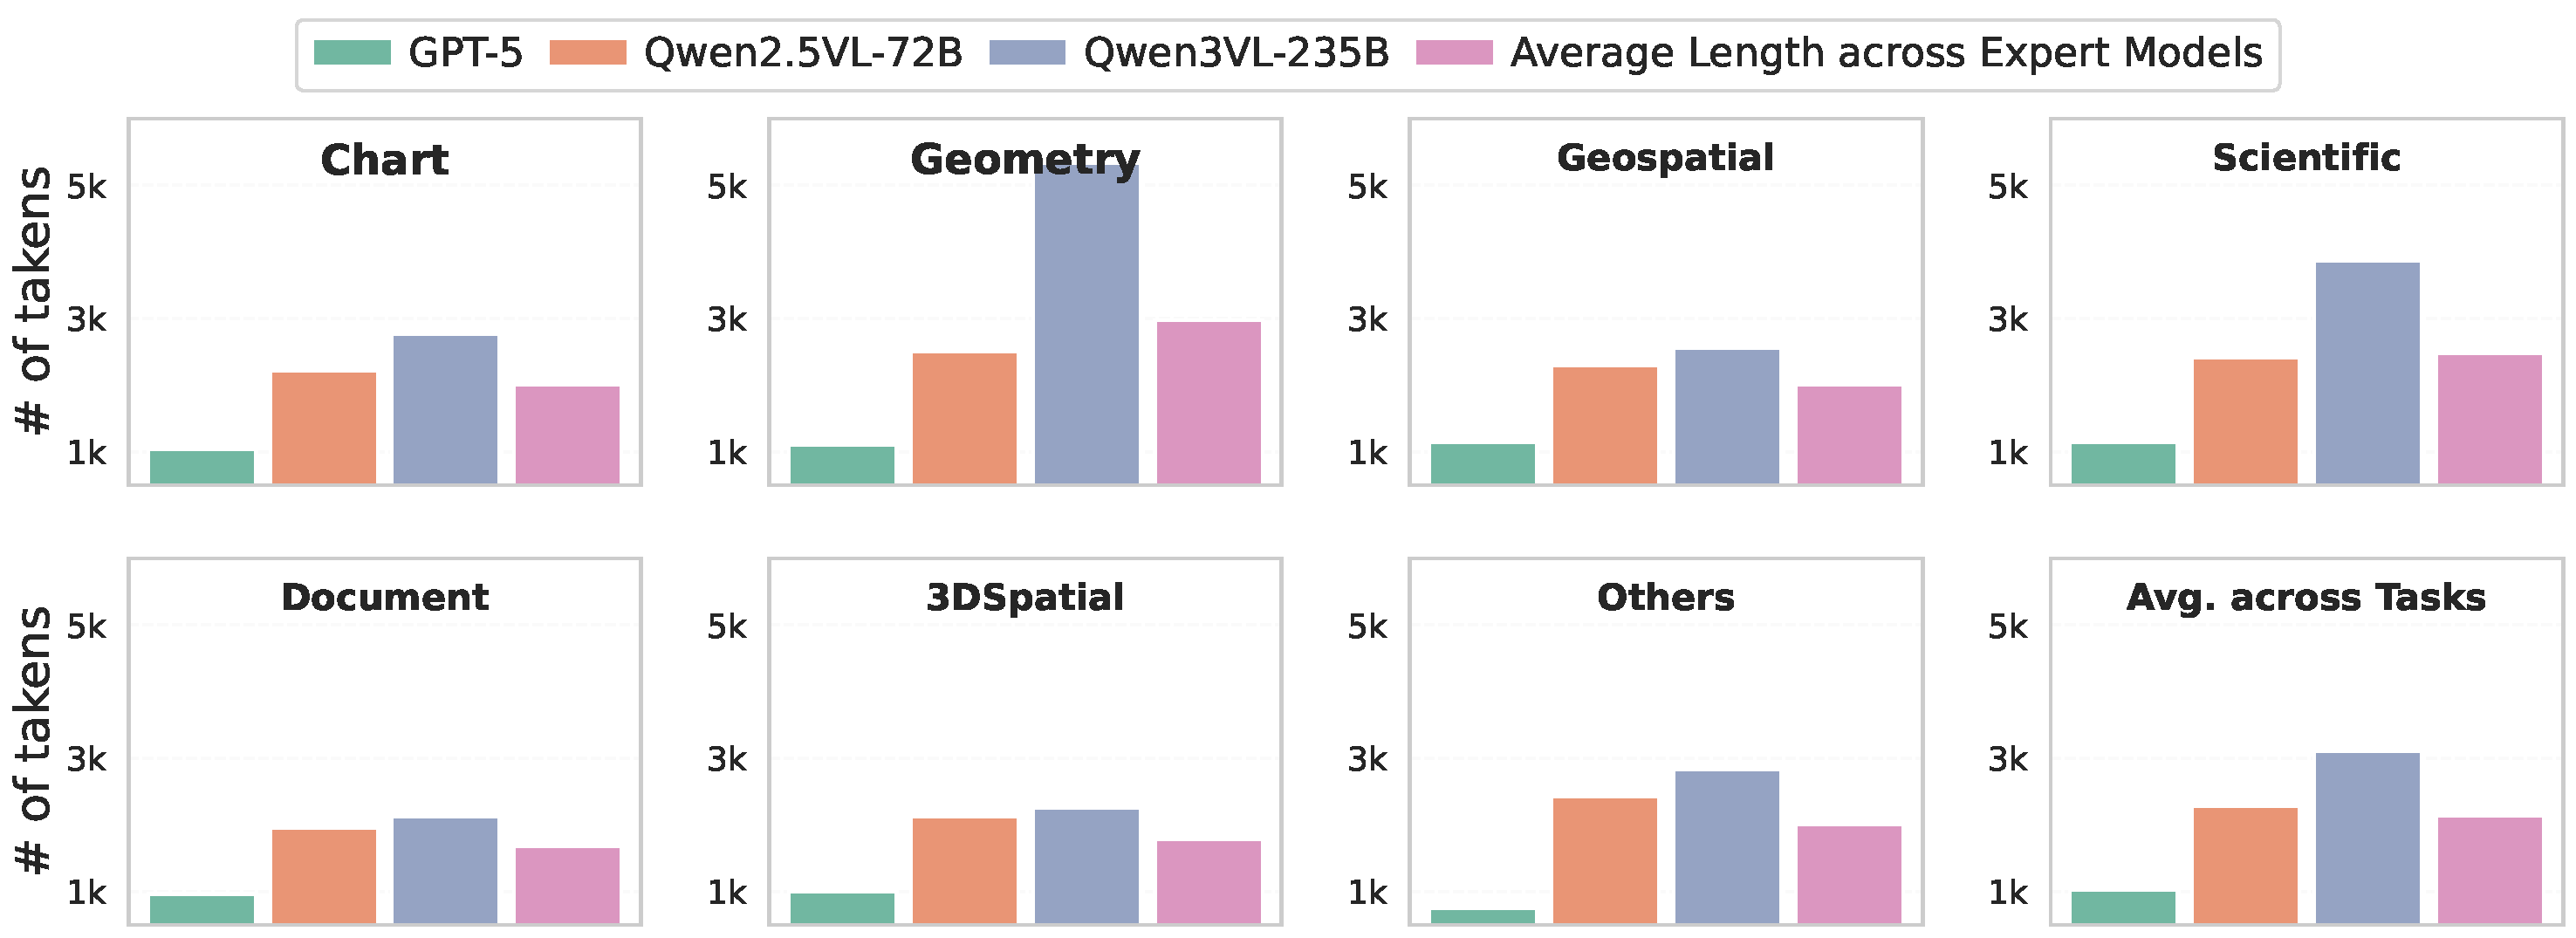
\includegraphics[width=\linewidth]{figure/traj-quality.pdf}
        \caption{Quality of expert thinking trajectories by length.}
        \label{fig:traj-quality}
    \end{minipage}
    \hfill
    \begin{minipage}[t]{0.27\linewidth}
        \centering
        
\includegraphics[width=\linewidth]{figure/error_analysis.pdf}
        \caption{Error analysis.}
        \label{fig:error-transfer}
    \end{minipage}
    % \vspace{-1ex}
\end{figure*}


\begin{figure}[t]
    \centering
    \begin{subfigure}[t]{0.49\linewidth}
        \centering
        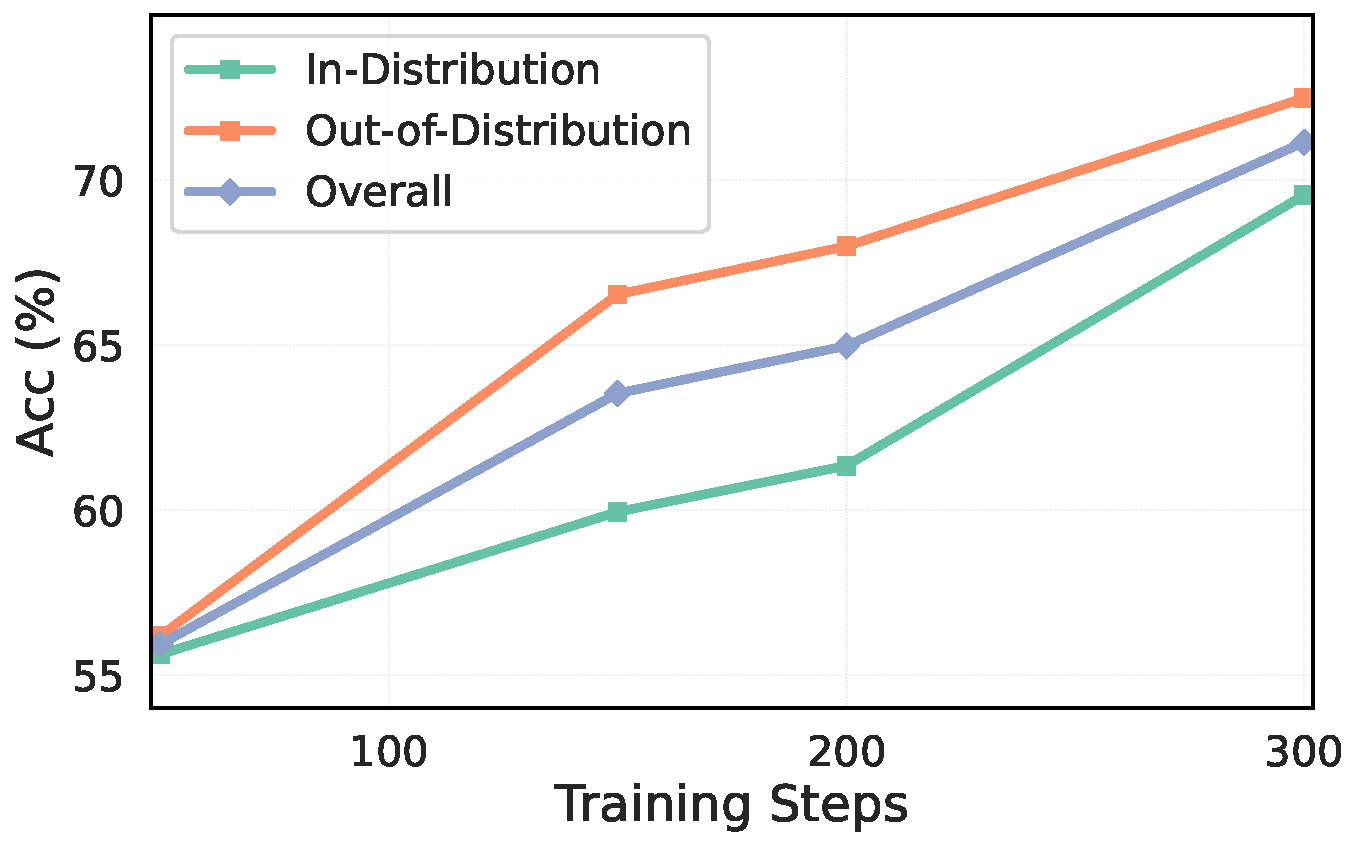
\includegraphics[width=\linewidth]{figure/epoch_plot.pdf}
        \caption{Training scaling}
        \label{fig:train-scale}
    \end{subfigure}
    \hfill
    \begin{subfigure}[t]{0.49\linewidth}
        \centering
    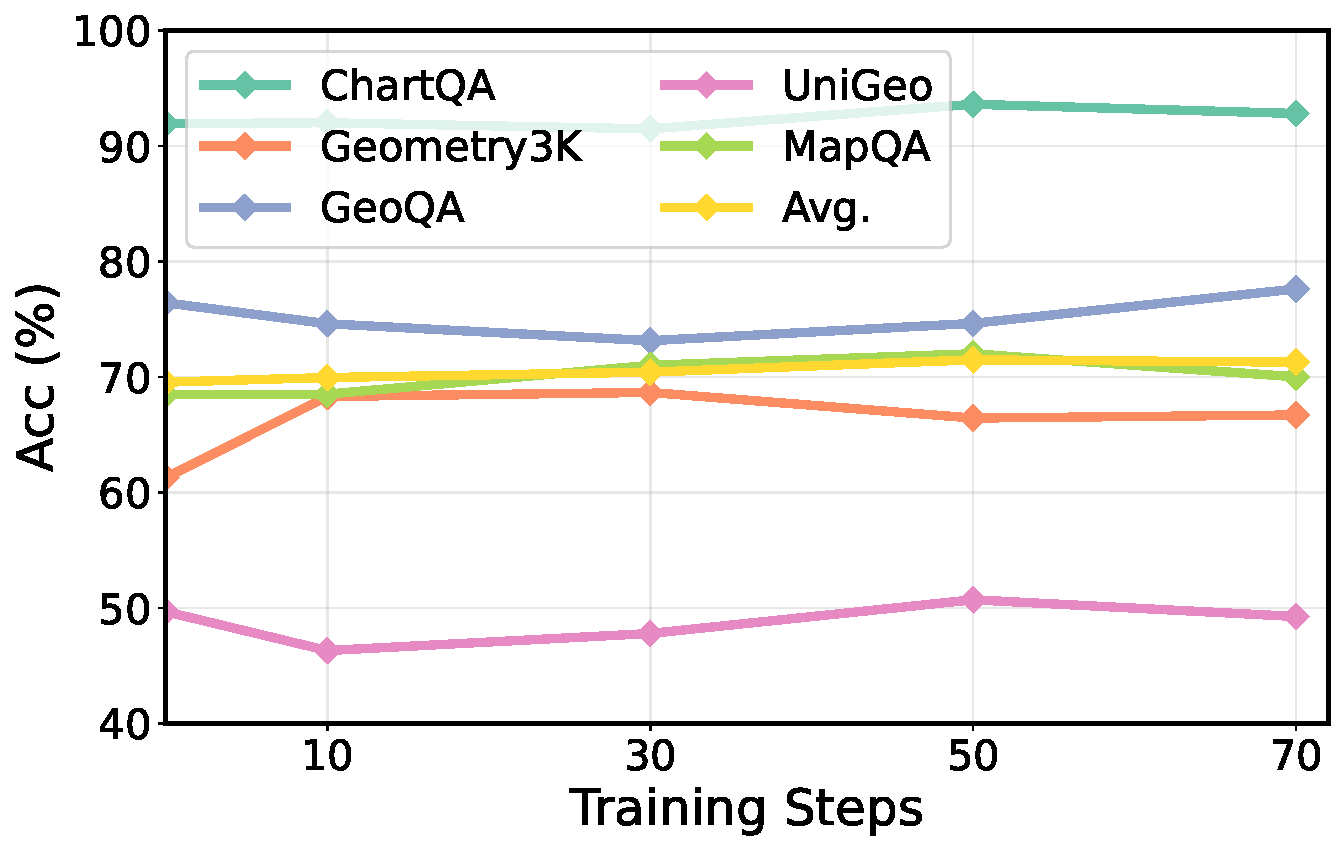
\includegraphics[width=\linewidth]{figure/tailpatch.pdf}
    \caption{Tailpatch}
    \label{fig:tailpatch}
    \end{subfigure}
    \caption{Training scaling from easy to hard.}
    \label{fig:scale}
    % \vspace{-2.5ex}
\end{figure}


\subsection{Additional Studies of \env{}}
\noindent \textbf{Data Diversity: Effect of Data Mixture.}
Figure~\ref{fig:adata-diversity} examines how task composition during RL shapes TIR. 
Single‑task training exhibits weak cross‑task transfer, especially across distinct domains such as ChartQA (chart understanding) and UniGeo (geometric reasoning), likely due to shifts in tool‑use schemas and argument distributions that narrow the learned policy’s coverage of the action space and impede general TIR. 
By contrast, multi-task training consistently improves generalization, indicating that exposure to a diverse task mixture during training is key to learning transferable TIR policies.

\noindent \textbf{Tool Diversity: Effect of Tool Mixture.}
Figure~\ref{fig:tool-diversity} analyzes how tool composition during RL shapes TIR using ChartMoE as an example. Training \emph{exclusively} with chart-understanding tools leaves chart-centric tasks (ChartQA; to a lesser extent, MapQA) largely unchanged, but transfers poorly to tasks with different tool affordances (UniGeo). Similar to data mixture, exposure to heterogeneous tool schemas and argument formats also mitigates over‑specialization and broadens the learned action policy.

\noindent \textbf{Reasoning Trajectory Quality.}
We assess the \emph{quality} of expert trajectories (GPT-5, Qwen2.5VL-72B, Qwen3VL-235B) using token length as a simple proxy in Figure~\ref{fig:traj-quality}. As expected, longer trajectories during the SFT warm‑up establish better behavior prior, thus contribute to higher performance after RL (Figure~\ref{fig:effect-of-traj-quality}). Note that commercial APIs such as GPT‑5 often do not expose full intermediate reasoning, yielding significantly shorter trajectories and weaker gains from agentic RL under the same training recipe.

\noindent \textbf{Tail-Patch Curriculum.}
To overcome the performance plateau, we adopt an easy-to-hard curriculum that \emph{tail-patch} training with increasingly challenging samples.
We use rollout pass rates from the previous checkpoint as a dynamic difficulty signal and isolate \emph{hard-but-learnable} instances with pass rates in $[0.125, 0.375]$.
Continuing RL exclusively on this high-difficulty slice pushes performance beyond the initial convergence point (69.54\% $\rightarrow$ 71.27\%) (Figure~\ref{fig:scale}).
This suggests a general principle: focusing the optimization budget on the \emph{frontier of competence}—cases where the model is uncertain yet occasionally succeeds—sharpens long-horizon reasoning and delivers fine-grained gains.


\subsection{Error Analysis and Case Study}
\noindent \textbf{Error Analysis.}
We re‑evaluate error patterns on the same 500 samples from Table~\ref{tab:error-def} after InternVL3-8B (left in Figure~\ref{fig:error-transfer}) training with \env{} (right). Agentic training within \env{} markedly resolves the majority of tool-call and reasoning failures observed in base models.

\begin{figure}[t]
    \centering
    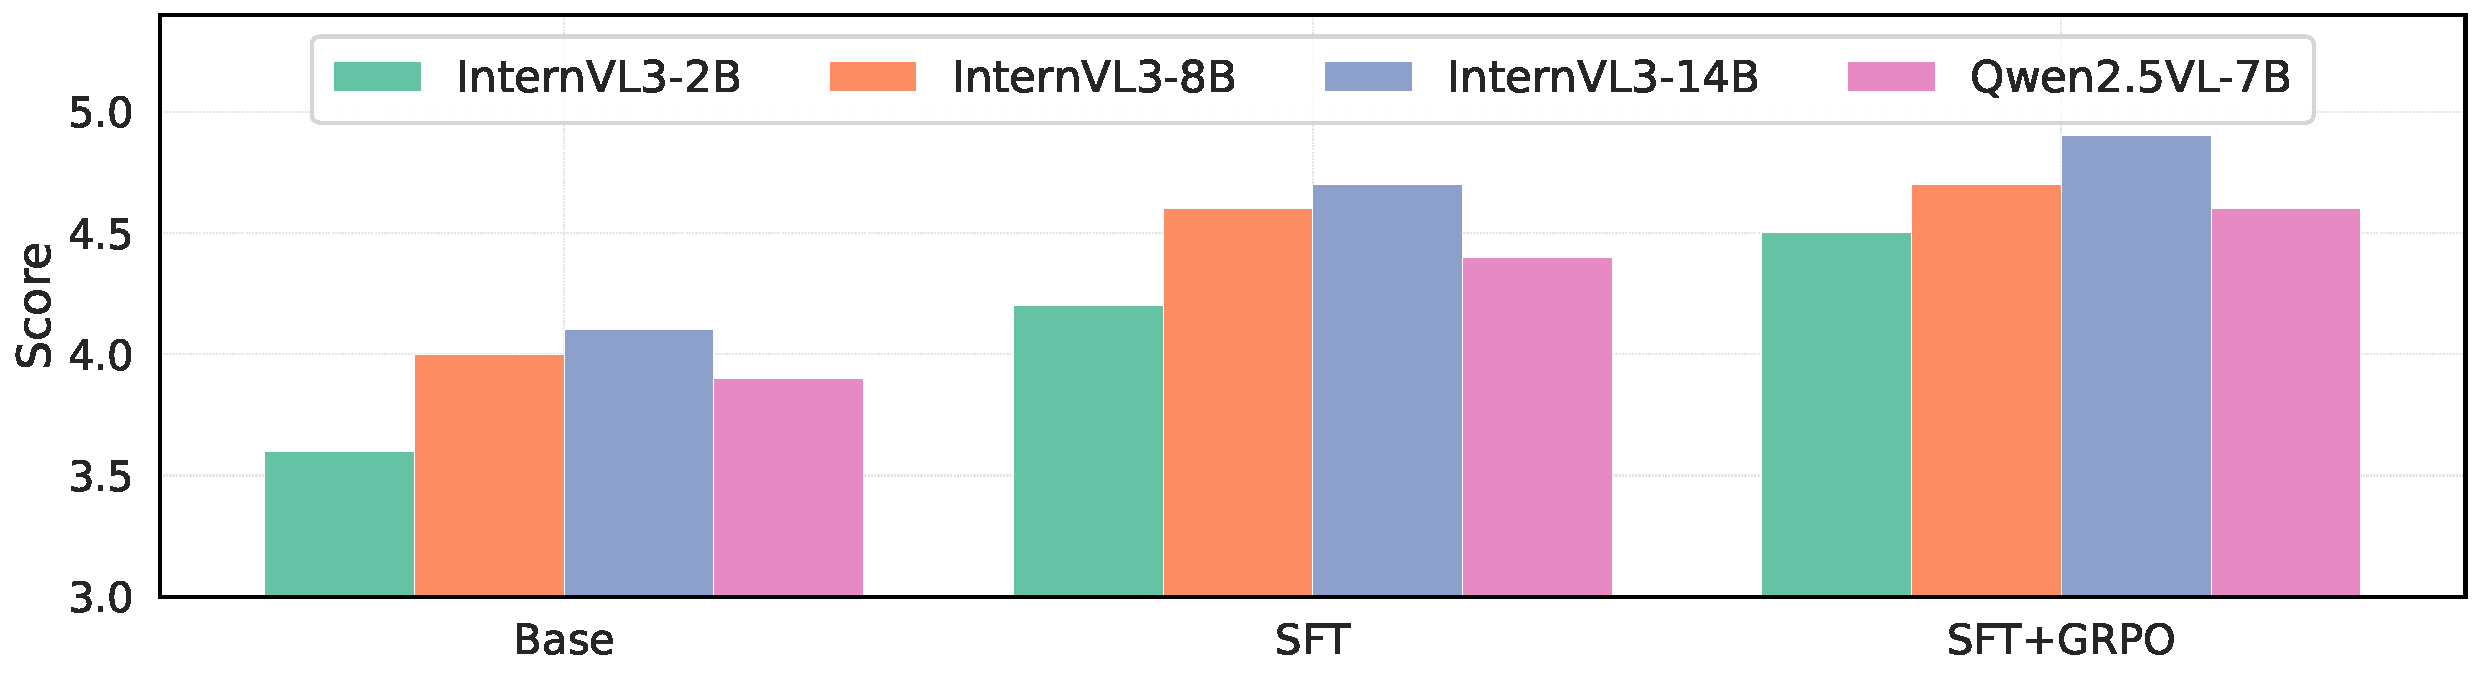
\includegraphics[width=\linewidth]{figure/human-study.pdf}
    \caption{Human study on trajectory quality.}
    % \vspace{-2ex}
    \label{fig:human-study}
\end{figure}

\noindent \textbf{Human Study for Trajectory Quality.}
As TIR trajectories are a key component of \env{}, we evaluate the quality of the generated interleaved tool-use and reasoning steps. Figure~\ref{fig:human-study} reports average human ratings (1–5 scale) over 40 randomly sampled solution trajectory per dataset. We observe that both training stages significantly improve TIR across tasks and model sizes.



\begin{table*}[t]
\centering
\renewcommand\arraystretch{0.95}
\caption{Case studies on geometric reasoning tasks with \ours-8B trained in \env{}.}
\resizebox{\linewidth}{!}{
    \begin{tabular}{p{1.8cm}p{21cm}}
    % \begin{tabular}{p{2cm}p{18cm}}
       \toprule
       \multicolumn{2}{l}{\textbf{Case Study 1}: Find m $\angle$ R. \textbf{Answer: A}: 58} \\
       % \midrule
        % \bf Q / A & who hosted and won the inagural world cup / Uruguay  \\
        \midrule
        \bf \multirow{6}{*}{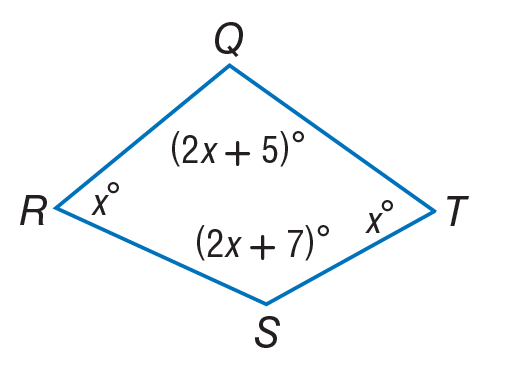
\includegraphics[width=\linewidth]{figure/casestudy/2489_img_diagram.png}} & \textbf{InternVL3-8B-Tool}: \textcolor{blue}{<tool\_call>}\{"tool": "multimath", "task": "solve\_the\_problem", "arguments": \{"image\_url": <image\_url>, "data": \{\textcolor{red}{"image/png": base64, iVBORw0KGgoAAAANSUhEUgAAAOAAAAHCAIAAADYXJpAAAAA3NCSV $\cdots$ (including long base64 image data)}\}\}\textcolor{blue}{</tool\_call>} \hfill \colorbox{red!15}{\textbf{Tool Call Error}: \emph{Invalid Arguments}. (\ding{56})} \\
        & \textbf{\ours}: \textcolor{blue}{<tool\_call>}\{"tool": "gllava", "task": "solve", "arguments": "Find m $\angle R$ from the diagram: a diamond-shaped quadrilateral with vertices R (left), Q (top), T (right), S (bottom). Angles labeled: at $R = x^\circ$, at $T = x^\circ$, at $Q = (2x+5)^\circ$, at $S = (2x+7)^\circ$."\}.\textcolor{blue}{</tool\_call>} \hfill \colorbox{green!15}{\textbf{Tool Call}: \emph{Correct} (\ding{51})} \\
        \midrule
        \multicolumn{2}{p{23cm}}{\textbf{Case Study 2}: As shown in the figure, in $\odot O$, $AB$ is a diameter and $CD$ is a chord. $AB \perp CD$, with the foot of the perpendicular at point $E$. Connect $CO$ and $AD$. If $\angle BOC = 30^\circ$, then the degree measure of $\angle BAD$ is ( ). \textbf{Answer: 15$^\circ$}} \\
        \midrule
        \bf \multirow{6}{*}{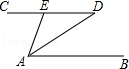
\includegraphics[width=\linewidth]{figure/casestudy/102.png}}  & \textbf{InternVL3-8B-Tool}: $\cdots$\textasciigrave\textasciigrave\textasciigrave output $\cdots$Step 12 (Property of isosceles triangle): $\angle BAD = \angle OAD$. Answer: $\angle BAD = 15^\circ$.\textasciigrave\textasciigrave\textasciigrave \textcolor{blue}{<think>} Alright, \textcolor{red}{let's tackle this geometry problem step by step}. $\cdots$ But according to the tool output, the answer is 15 degrees, which is option D. \textcolor{red}{But my computation also says the answer is 52.5 degrees. So the answer is closer to C}. \textcolor{blue}{</think>}$\cdots$ \hfill \colorbox{red!15}{\textbf{Correct Tool, Wrong Reasoning}: \emph{Incorrect reasoning to answer.}. (\ding{56})}\\
        & \textbf{\ours}: $\cdots$ \textasciigrave\textasciigrave\textasciigrave output $\cdots$Step 12 (Property of isosceles triangle): $\angle BAD = \angle OAD$. Answer: $\angle BAD = 15^\circ$.\textasciigrave\textasciigrave\textasciigrave\textcolor{blue}{<think>} \textcolor{green!50!black}{$\cdots$Based on the previous verification and tool output, I can analyze and provide the answer of $15^\circ$.}\textcolor{blue}{</think> <answer>}15$^\circ$\textcolor{blue}{</answer>}. \hfill \colorbox{green!15}{\textbf{Reasoning}: \emph{Correct} (\ding{51})} \\
        \midrule
        \multicolumn{2}{p{23cm}}{\textbf{Case Study 3}: $AB || CD$. Line $EF$ intersects $AB$ at point $E$ and intersects $CD$ at point $F$. $EG$ bisects $\angle BEF$ and intersects $CD$ at point $G$. If $\angle 1 = 50^\circ$, then $\angle 2$ equals ( ). Choices:A: $50^\circ$B: $60^\circ$C: $65^\circ$D: $90^\circ$. \textbf{Answer: C: 90$^\circ$.}} \\
        \midrule
        \bf \multirow{7}{*}{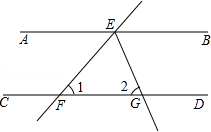
\includegraphics[width=\linewidth]{figure/casestudy/1.png}} & \textbf{\ours}: \textcolor{blue}{<think>} $\cdots$ \textcolor{green!50!black}{ChartMoE is appropriate because it is designed to analyze structured geometric diagrams, accurately reading angle labels, identifying parallel-line configurations, and aligning textual annotations with diagram elements. I will have it parse the diagram to confirm $AB||CD$, locate the transversal EF and the points E, F, G, and verify that EG bisects $\angle BEF$ while intersecting CD at G.} By interpreting the angles formed at E relative to BE and FE and using the parallel-line angle relations (corresponding, alternate interior, and consecutive interior angles), ChartMoE will relate $\angle 1$ to the angle between BE and EG, propagate the bisector relation to $\angle BEF$, and then deduce the measure of $\angle 2$ at the intersection of EF and CD from the resulting angle measures. Finally, it will align that computed value with the provided choices. Therefore, I will call chartmoe now.\textcolor{blue}{</think><tool\_call>}\{"tool": "chartmoe", "task": "analyze"\}\textcolor{blue}{</tool\_call>} $\cdots$ \hfill \colorbox{green!15}{\textbf{New Tool Selection}: \emph{Expected G-LLaVA but got ChartMoE.} (\ding{51})}\\
        \midrule
        \multicolumn{2}{p{23cm}}{\textbf{Case Study 4}: Find X Z. \textbf{Answer: D: 34.}} \\
        \midrule
        \bf \multirow{16}{*}{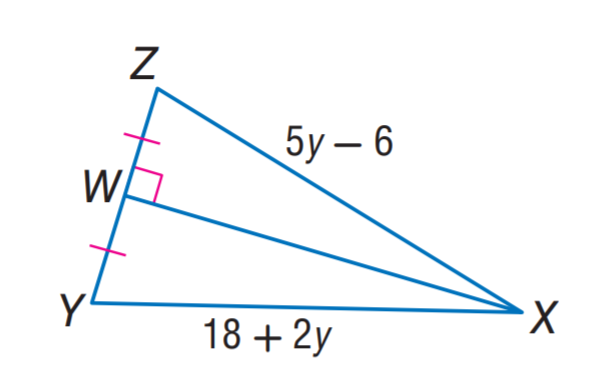
\includegraphics[width=\linewidth]{figure/casestudy/2430_img_diagram.png}} & \textbf{InternVL3-8B-Tool}: \textcolor{blue}{<tool\_call>}\{"tool": "multimath", "task": "Solve the problem", "arguments": \{"image": "<image>", "question": "Find X Z. $\cdots$"\}\}\textcolor{blue}{</tool\_call>}\textasciigrave\textasciigrave\textasciigrave output $\cdots$ Step 5 (Simplify the equation): $XZ^2 = 29y^2 + 12y + 360.$\textbackslash nAnswer: \textbackslash boxed\{$29y^2 + 12y + 360$\}\textasciigrave\textasciigrave\textasciigrave\textcolor{blue}{<think>} $\cdots$ But as we saw earlier, this leads to a quadratic with no real solutions.\textbackslash n \textcolor{red}{Wait, maybe I made a mistake in the tool output. Let me double-check the steps: \textbackslash n Step 3: $XZ^2 = (5y - 6)^2 + (18 + 2y)^2 = 25y^2 - 60y + 36 + 324 + 72y + 4y^2 = 29y^2 + 12y + 360$. That seems correct.}\textbackslash n $\cdots$ Step 5: Simplify the equation: $XZ^2 = 29y^2 + 12$\textcolor{blue}{</think><answer>} \textbackslash boxed\{C\}.\textcolor{blue}{</answer>} \hfill \colorbox{red!15}{\textbf{Tool Output Error}: \emph{Incorrect reasoning to answer.}. (\ding{56})}\\
        & \textbf{InternVL3-8B-Reasoning}: <think> Alright, let's tackle this problem step by step. First, I notice that triangle WYZ is a right triangle because it has a right angle at W. $\cdots$ Using the Pythagorean theorem again:\textbackslash n$XZ^2 = WZ^2 + XY^2$\textbackslash n$XZ^2 = 34^2 + 34^2$, $XZ^2=2312$, $XZ=\sqrt{2312}=34*\sqrt{2}$\textbackslash n Therefore, the length of XZ is $34\sqrt{2}$.\textbackslash n</think>\textbackslash n<answer>$34\sqrt{2}$</answer>" \hfill \colorbox{red!15}{\textbf{No Tool-use}: \emph{Insufficient capability to answer.}. (\ding{56})}\\
        & \textbf{\ours}: \textcolor{blue}{<think>} $\cdots$ \textcolor{green!50!black}{Multimath is appropriate because} $\cdots$ I will read from the image that $WX\perp ZX$ $\cdots$. \textcolor{green!50!black}{Multimath will translate these visual relations into algebraic constraints}, $\cdots$. \textcolor{blue}{</think><tool\_call>}\{"tool": "multimath", "task": "solve"\}\textcolor{blue}{</tool\_call>}\textasciigrave\textasciigrave\textasciigrave output $\cdots$ Step 10 (Calculate the value of XZ): $XZ = 18 + 2y = 18 + 2(\frac{6}{5}) = 18 + \frac{12}{5} = \frac{90}{5} + \frac{12}{5} = \frac{102}{5} = 20.4$. \textasciigrave\textasciigrave\textasciigrave \textcolor{blue}{<think>} Looking at the tool's solution, it set up the equation $25y^2 - 60y + 36 = 0$ and solved to get $y = 6/5$. Let me verify this step by step. $\cdots$ \textcolor{green!50!black}{Wait, let me check if this makes sense geometrically.} $\cdots$ Actually, if the tick marks indicate equal segments, shouldn't we have $5y - 6 = 18 + 2y$? Let me solve this: $5y - 6 = 18 + 2y 3y = 24 y = 8$ With $y = 8$, let's calculate XZ. If $XZ = 18 + 2y$, then: $XZ = 18 + 2(8) = 18 + 16 = 34$. \textcolor{green!50!black}{Hmm, that's different from the tool's answer of $20.4$. Let me reconsider.} $\cdots$ \textcolor{green!50!black}{The tool calculated 20.4, but based on the equal segment marks, the answer is $34$.}\textcolor{blue}{</think><answer>}$34$\textcolor{blue}{</answer>}" \hfill \colorbox{green!15}{\textbf{TIR}: \emph{correct} (\ding{51})} \\
       \bottomrule
    \end{tabular}
%\end{center}
}
 % \vspace{-1ex}
	\label{tab:case_study}
\end{table*}


\noindent \textbf{Case Studies.}
Table~\ref{tab:case_study} presents four case studies illustrating the capabilities acquired through agentic training in \env{}: (i) schema‑ and argument‑correct \emph{tool invocation}; (ii) \emph{post‑tool reasoning} that grounds the final answer in tool outputs; (iii) \emph{cross‑tool generalization} that repurposes atypical yet useful tools (\eg, applying ChartMoE on geometry problems); and (iv) \emph{robustness to imperfect tool outputs}, where the agent identifies and exploits partial signals over multiple turns to complete multi‑step reasoning. 

